\section{User Manual}

\subsection{Sign in}
\begin{figure}[H]
	\centering
	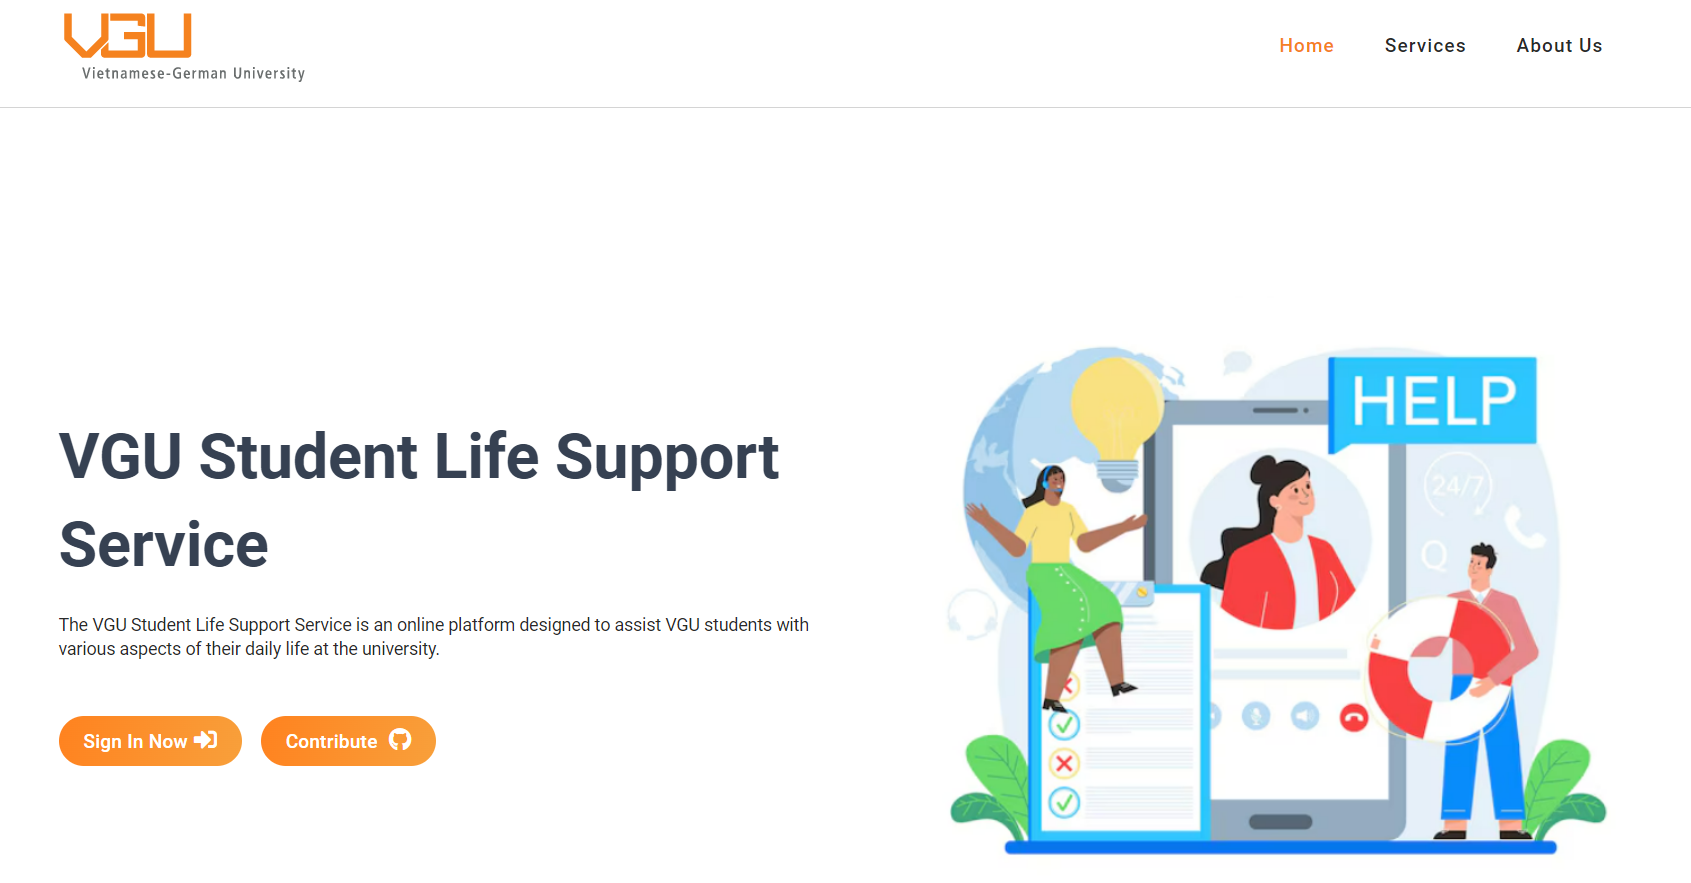
\includegraphics[width=1.\linewidth]{graphics/gui/user/landing}
	\caption{Landing page}
	\label{fig:landing}
\end{figure}

In the landing page of the service, navigate to Login page by clicking "Sign In Now"


\begin{figure}[H]
	\centering
	\begin{minipage}{.5\textwidth}
		\centering
		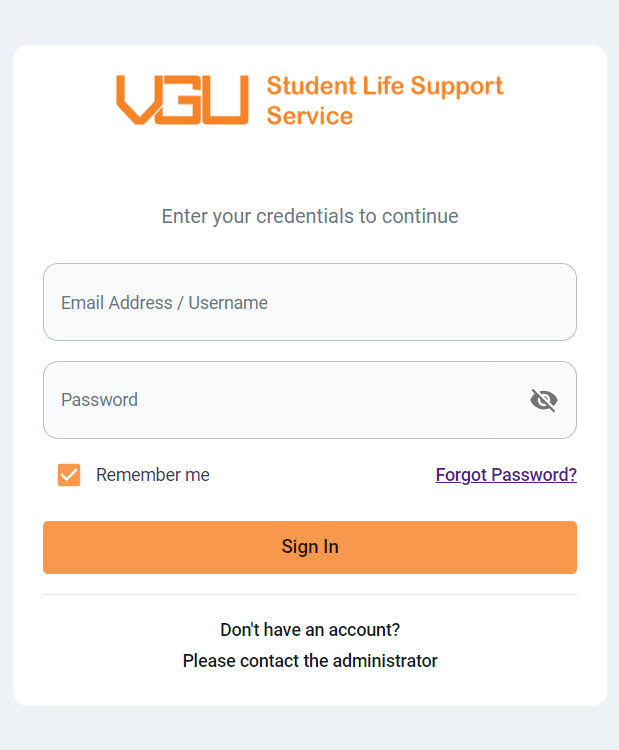
\includegraphics[width=.9\linewidth]{graphics/gui/user/login.png}
		\captionof{figure}{Sign in Form}
		\label{fig:gui-login}
	\end{minipage}%
	\begin{minipage}{.5\textwidth}
		\centering
		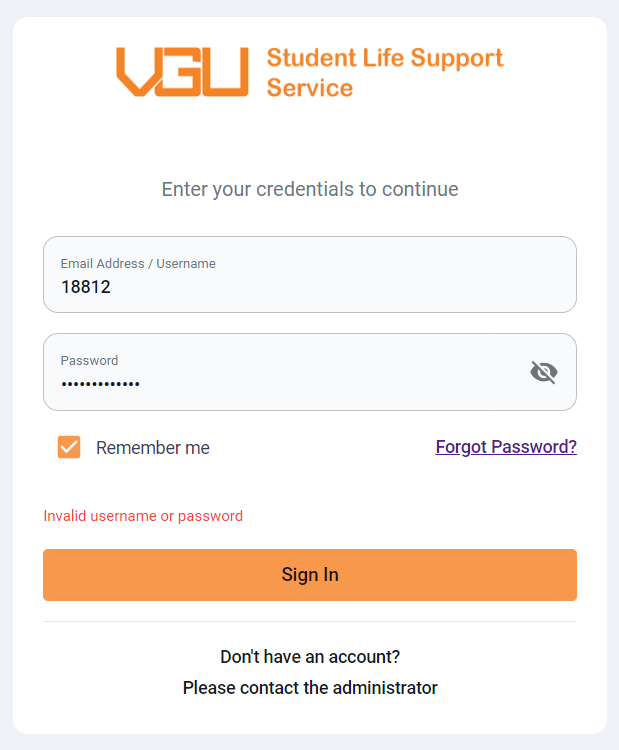
\includegraphics[width=0.9\linewidth]{graphics/gui/user/login-error.png}
		\captionof{figure}{Failed Sign in attempt}
		\label{fig:gui-login-failed}
	\end{minipage}
\end{figure}



To access the service, input your username (or email) and password, then click on the sign-in button (refer to Figure \ref{fig:gui-login}). If you provide incorrect credentials, a warning message will appear, indicating that you need to correct either your username or password (Figure \ref{fig:gui-login-failed}).





\subsection{Forgot password}

%In case of forgetting your password, you can reset it by clicking 'Forgot Password?' of the 'Sign in' form (see Firgure \ref{fig:gui-login}). Then, enter your the email in the 'Forgot Password' form adn click 'Reset Password' (Figure \ref{fig:gui-forgot-pass})

If you forget your password, you can initiate a reset by selecting the 'Forgot Password?' option on the 'Sign in' form (refer to Figure \ref{fig:gui-login}). Subsequently, provide your email address in the 'Forgot Password' form and click on 'Reset Password' (see Figure \ref{fig:gui-forgot-pass}).

\begin{figure}[H]
	\centering
	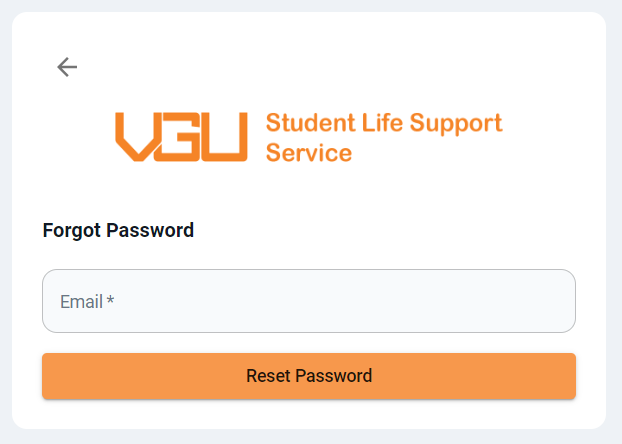
\includegraphics[width=0.7\linewidth]{graphics/gui/user/reset-pass.png}
	\caption{Reset password form}
	\label{fig:gui-forgot-pass}
\end{figure}



If your email is associated with an account in the system, a success notification will appear, and password reset instructions will be sent to your email (Figure \ref{fig:gui-reset-pass-success}, \ref{fig:gui-email-reset-pass}).  Conversely, if the email is not found in the system, a failure notification will indicate that the email does not exist (Figure \ref{fig:gui-reset-pass-failed}).

\begin{figure}[H]
	\centering
	\begin{minipage}{.5\textwidth}
		\centering
		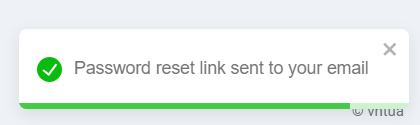
\includegraphics[width=.9\linewidth]{graphics/gui/user/reset-pass-success.png}
		\captionof{figure}{Reset password successfully}
		\label{fig:gui-reset-pass-success}
	\end{minipage}%
	\begin{minipage}{.5\textwidth}
		\centering
		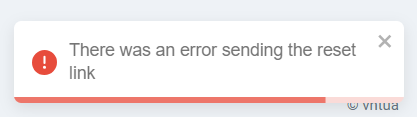
\includegraphics[width=0.9\linewidth]{graphics/gui/user/reset-pass-failed.png}
		\captionof{figure}{Reset password failed}
		\label{fig:gui-reset-pass-failed}
	\end{minipage}
\end{figure}


\begin{figure}[H]
	\centering
	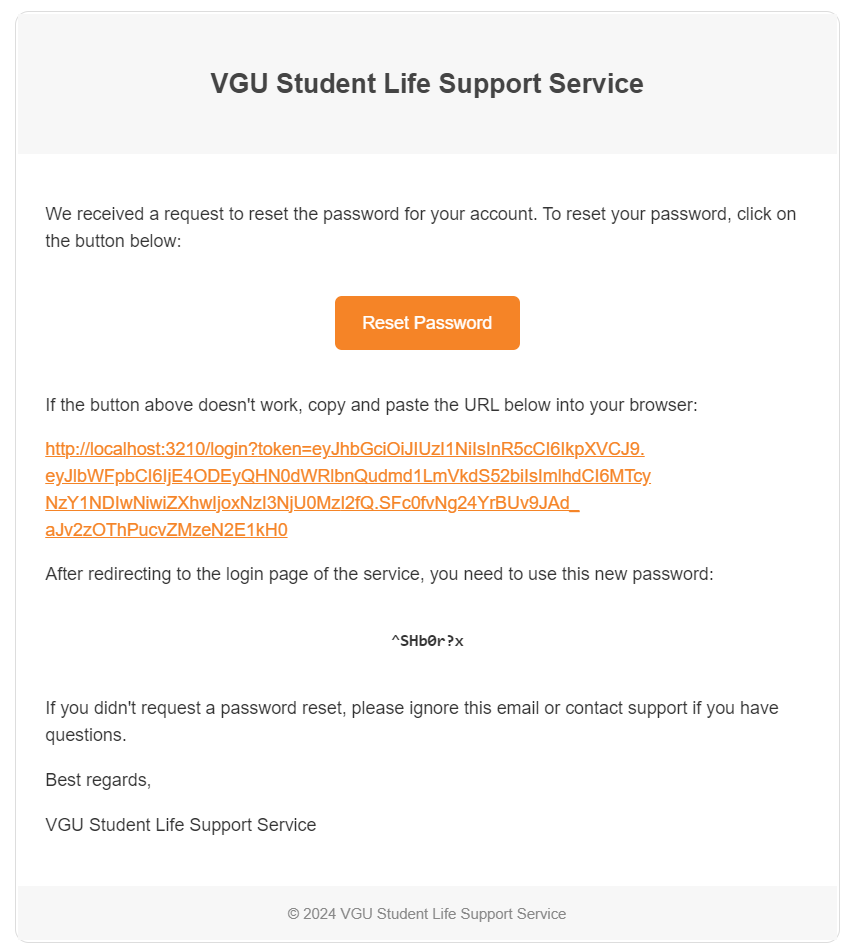
\includegraphics[width=0.8\linewidth]{graphics/gui/user/email-reset.png}
	\caption{Reset password email instructions}
	\label{fig:gui-email-reset-pass}
\end{figure}




